\documentclass[10pt,a4paper]{amsart}

\usepackage[]{graphicx} 
\usepackage[]{url} 
\usepackage[]{program} 
\usepackage[]{caption} 
\usepackage[]{subcaption} 
\usepackage[]{hyperref} 
\usepackage[]{cleveref} 

\usepackage[]{libertine} 
\usepackage[T1]{fontenc} 

\title[Solving the Poisson-equation in one dimension]{
  Solving the Poisson-equation in one dimension. \\
  \hrulefill\fbox{FYS3150}\hrulefill
}
\author[Ivar Stangeby]{
  Ivar Stangeby \\
  \href{https://github.com/qTipTip/FYS3150/projects/project_1/}{\texttt{github.com/qTipTip/FYS3150} }
}
\begin{document}

  \begin{titlepage}
\begin{abstract}
  In this project we examine and solve the Poisson equation in one dimension.
  We consider various numerical methods for solving the discretized
  differential equation and compare their numerical efficiency.
\end{abstract}
  \maketitle
  
  \begin{figure}[h!]
    \centering
    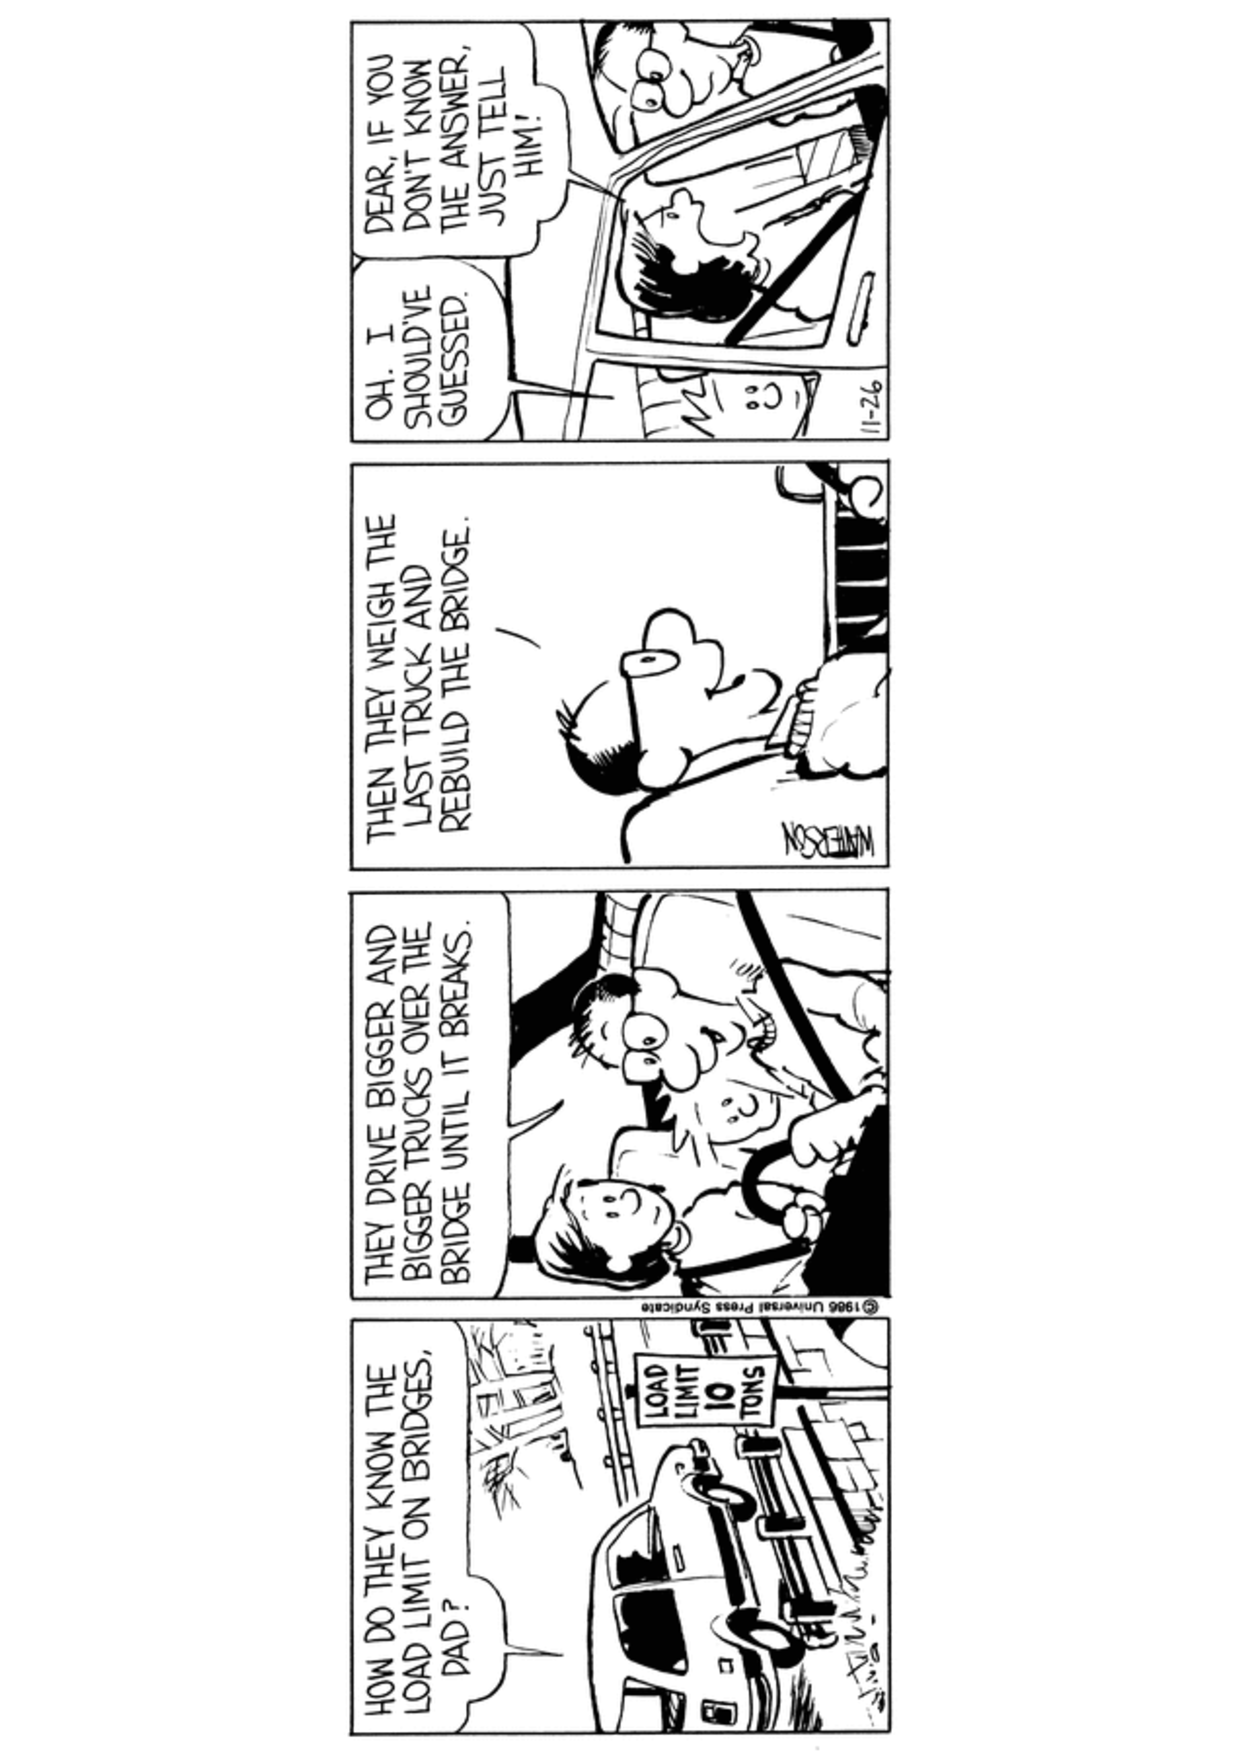
\includegraphics[angle=270, width=0.9\linewidth]{c_h.pdf}
  \end{figure}
  \tableofcontents
  \end{titlepage}

  \section{Introduction}
  \label{sec:introduction}

  In this project we are tasked with solving the one-dimensional Poisson
  equation.  One can look at the project as consisting of three parts.
  Analytical examination of the problem, numerical solution to the problem, and
  lastly, comparing our numerical results to our expectations in the first part.
  
  We start by deriving the three point approximation to the second
  derivative of a function $f$.  We then use this approximation to show that we
  can rewrite the set of equations as a matrix equation. Our task at hand is
  then to solve this matrix equation using some algorithm, which in this case
  is going to be the tridiagonal matrix algorithm (TDMA). We will analyze this
  algorithm to figure out what kind of results we can expect and we will
  compare this with the standard Gaussian elimination and LU decomposition
  methods. 

  We then implement our devised algorithm and solve our system for various
  grid-resolutions and compare our results with the closed form solution of our
  given problem. We will do this visually by plotting the analytical solution
  against the numerical solution.

  Lastly, we want to examine the relative error that occurs for various step
  sizes and extract the largest relative error over the grid for different
  resolutions. The motivation behind this is to figure out which resolution
  (step size) gives the most optimal results.  We then compare this to the
  expectations from part 1.


  \section{Formulating the problem}
  \label{seq:formulating}
  
  \subsection{Physical background}
  \label{sub:physical_background}
  
  The poisson-equation in three dimensions read
  \begin{equation}
    \notag
    \nabla^2\Phi = -4\pi\rho(\mathbf r) 
  \end{equation}
  where $\nabla^2$ is the Laplacian-operator. In three dimensions it is
  expressed using spherical coordinates. In this project however, we are going
  to assume that $\Phi$ and $\rho$ are spherically symmetric which essentially
  mean that the whole equation reduces to a one-dimensional problem in the
  radius $r$. Writing out the laplacian for a spherically symmetric system we
  get
  \begin{equation}
    \notag
    \nabla^2 = \frac{1}{r^2}\frac{d}{d2}\left( r^2 \frac{d}{dr} \right).
  \end{equation}
  If we substitute $\Phi(r) = \phi(r)/r$ our poisson-equation then reads
  \begin{equation}
    \notag
    \frac{d^2\phi}{dr^2} = -4\pi r \rho(r).
  \end{equation}
  The motivation behind this substitution is to ensure that we achieve the
  Dirichlet boundary conditions we want.

  We finally let $\phi \rightarrow u$ and $r \rightarrow x$, and the equation
  now reads
  \begin{equation}
    \label{eq:diff_eq}
    -u''(x) = f(x).
  \end{equation}
  The function $f$ is called the \textit{source term}, and in this project we
  are going to assume that $f(x) = 100e^{-10x}$. We can then compare our
  results with the closed form solution $u(x) = 1 - (1-e^{-10})x -e^{-10x}$.
  \Cref{eq:diff_eq} naturally gives rise to the need of a numerical
  approximation to the second derivative of a function $u$.

  \subsection{Approximating the second derivative}
  \label{sub:approximating_the_second_derivative}
  
  Writing out the Taylor-expansion of a function $f : \mathbb{R} \rightarrow
  \mathbb{R} $ we get
  \begin{equation}
    \notag
    f(x) = \sum^{\infty}_{i=0} \frac{f^{(n)}(a)}{n!}(x - a)^n.
  \end{equation}

  If we examine that partial sums $T_n$ of this series we are truncating the
  exact expansion at some $n$. Note that $f(x) = \lim_{n \rightarrow \infty}
  T_n$.
  \begin{equation}
    \notag
    T_n(x) = \sum^{n}_{i=0} \frac{f^{(n)}(a)}{n!}(x-a)^n.
  \end{equation}
  By doing this, we are essentially approximating our function $f$ at a point
  $x$, and we are introducing a truncation error. We evaluate $T_n$
  around $x = a$ at the point $x \pm h$ and achieve
  \begin{equation}
    \notag
    T_n(x\pm h) = \sum^{n}_{i=0} \frac{f^{(n)}(x)}{n!}h^n.
  \end{equation}

  Setting $n = 2$ we obtain a term containing the second derivative of $f$,
  \begin{equation}
    \notag
    T_2(x \pm h) = f(x) \pm f'(x)h + \frac{f''(x)}{2}h^2,
  \end{equation}
  and we now write out the sum of $T_2(x+h)$ and $T_2(x-h)$. This yields
  \begin{align*}
    \notag
    f(x + h) + f(x-h) &= T_2(x + h) + T_2(x - h) + \mathcal{O}(h^4) \\
    &= 2f(x) + f''(x)h^2 + \mathcal{O}(h^4)
  \end{align*}
  which when solved for $f''(x)$ is equal to
  \begin{equation}
    \label{eq:diff_app}  
    f''(x) = \frac{f(x+h) - 2f(x) + f(x-h)}{h^2}  + \mathcal{O}(h^2).
  \end{equation}

  This equation is the one we will employ during the solution of the linear
  system. Note that $\mathcal{O}(h^2)$ is just shorthand for the truncation
  error introduced by setting $n = 2$. It  is an error-function that runs like
  $h^2$, however we will take the approximation, so ignoring this error-term.
  We will later compare the results for various values of $h$. 

  \subsection{System of linear equations}
  \label{sub:system_of_linear_equations}
  
  We want to solve \cref{eq:diff_eq} over a discrete set of $n$ distinct points
  $\left\{ x_i \right\}_{i=1}^n$ where $x_i = ih$ over the interval $[0, 1]$.
  We define the step length $h = 1 / (n+1)$ and it then follows that $x_0 =
  0$ and $x_{n+1} = 1$.

  If we now write out \cref{eq:diff_eq} using our approximation to the second
  derivative, namely \cref{eq:diff_app}, and denote the discretized
  approximation to $u$ at a point $x_i$ as $v_i$ then we achieve the following
  for the discrete point $x_i$:
  \begin{equation}
    \notag
    -\frac{v_{i+1} - 2v_i + v_{i-1}}{h^2} = f_i \text{ for all } i = 1, \ldots, n,
  \end{equation} 
  where $f(x)$ is the source term. Note that we write $f(x_i) = f_i$.  In
  preparation for the next step we multiply through by $h^2$.
  \begin{equation}
    \label{eq:set_eq}
    -v_{i+1} + 2v_i - v_{i-1} = h^2f_i \text{ for all } i = 1, \ldots, n,
  \end{equation} 
  We now observe that \Cref{eq:set_eq} along with the set of $i$'s define a set
  of $n$ linear equations. Writing them out, we notice a pattern:
  \begin{gather*}
    \label{eq:system}
    -v_2 + 2v_1 - v_0 = h^2f_1 \\
    -v_3 + 2v_2 - v_1 = h^2f_2 \\
                      \vdots \\
    -v_{n} + 2v_{n-1} - v_{n-2} = h^2f_{n-1} \\
    -v_{n+1}+ 2v_n - v_{n-1} = h^2f_n \\
  \end{gather*}
  Remember that we only have $n$ equations and $n+2$ unknowns, hence the
  Dirichlet boundary conditions are key if we are to solve this system.

  This system can be rewritten in terms of a coefficient matrix $A$, a vector
  $\mathbf v$ consisting of the variables $v_i$, and a vector
  $\mathbf{\tilde{b}}$ that consists of $b_i = h^2f_i$. Our system is now
  reduced to a matrix equation
  \begin{equation}
    \label{eq:matrix}
    A \mathbf v = \mathbf{\tilde b}.
  \end{equation}
  Note that $A$ is an $n\times n$ matrix, which does not cover the end cases.
  Also note that $A$ is a tridiagonal matrix, because only the middle three
  diagonals are non-zero.
  
  \section{Solving the problem}
  \label{sec:solving_the_problem}
    
  In this section we examine the implementation specific details of this
  project.  We are now going to outline the algorithm known as the
  \textit{Thomas Algorithm}, or \textit{Tridiagonal Matrix
  Algorithm}.\cite{thomasalgo} The Tridiagonal Matrix Algorithm is a special case of LU-decomposition tailored to tridiagonal systems. Due to problems with getting the armadillo \textit{solve()} method to work, I will also implement the standard Gaussian algorithm for comparison.

  \subsection{Devising an algorithm}
  \label{sub:devising_an_algorithm}
  
  In order to solve this matrix equation involving a tridiagonal matrix there
  are several shortcuts we can take. First note that the matrix is sparse,
  i.e., that the number of non-zero elements scale as $\mathcal{O}(n)$. In our
  case, since the elements are all along the three main diagonals we can make
  significant cuts in the memory by only storing the three diagonals as
  vectors. This way we only have to store $3n$ of the elements, assuming we
  only work with vectors of length $n$.
  
  If we let $\mathbf a$, $\mathbf b$, $\mathbf c$ denote the three main
  diagonals with elements $a_i, b_i, c_i$ for $i = 1, \ldots, n$ respectively
  then \cref{eq:set_eq} can be written as
  \begin{equation}
    \notag
    a_iv_{i+1} + b_iv + cv_{i-1} = h^2 f_i = \tilde b_i.
  \end{equation}
  
  Our goal now is to use the first equation to eliminate $v_1$ from the second
  equation, then use the new modified second equation to eliminate $v_2$ from
  the third equation and so on. After doing this for all $n$ equations, the
  final equation is an equation in one variable, namely $v_{n}$, which can be
  used to solve the previous $n-1$ equations.  This is an algorithm in two
  steps, a forward sweep where we forward substitute, and then a backward sweep
  where we substitute back in to solve the equations.  This algorithm scales
  linearly in the number of grid points. We require $2n$ substitutions, so the
  algorithm runs in $\mathcal{O}(n)$.
  
  We now wish to decompose $A$ into two triangular matrices. We denote these by
  $L$ and $U$ respectively.  We can now write \cref{eq:matrix} in terms of
  these new matrices:
  \begin{equation}
    \label{eq:lu}
    L U \mathbf v = \mathbf{\tilde{b}},
  \end{equation}
  with 
  \begin{equation}
    \notag
    A = \begin{bmatrix}
      \lambda_1 & \ldots & \ldots & \ldots & \ldots & \ldots\\
      a_1 & \lambda_2 & \ldots & \ldots & \ldots & \ldots\\
      \ldots & \ldots & \ldots & \ldots & \ldots & \ldots\\ 
      \ldots & \ldots & \ldots & a_{n-1} & \lambda_{n-1} & \ldots\\
      \ldots & \ldots & \ldots & \ldots & a_{n} & \lambda_{n} \\
    \end{bmatrix}\cdot
    \begin{bmatrix}
      1 & \gamma_1 & \ldots & \ldots & \ldots & \ldots\\
      \ldots & 1 & \gamma_2 & \ldots & \ldots & \ldots\\
      \ldots & \ldots & \ldots & \ldots & \ldots & \ldots\\ 
      \ldots & \ldots & \ldots & \ldots & 1 & \gamma_{n-1} \\
      \ldots & \ldots & \ldots & \ldots & \ldots & 1 \\
    \end{bmatrix}
  \end{equation}
 
  We start by first solving $L\mathbf y = \mathbf{\tilde b}$. This gives us the
  equations
  \begin{align*}
    \label{eq:y}
    y_i = \begin{cases}
      \frac{\tilde b_i}{\lambda_i}, & i = 1 \\
      \frac{\tilde b_i - a_iy_{i-1}}{\lambda_i}, & i = 2, \ldots, n.
    \end{cases}
  \end{align*}
  And solving $U\mathbf v = \mathbf y$ yields:
  \begin{equation}
    \notag
    v_i = \begin{cases}
      y_i - \gamma_iv_{i+1}, & i = 1,\ldots, n-1 \\
      y_i, & i = n.
    \end{cases}
  \end{equation}
  All we need now is an expression for $\lambda_i$ and $\gamma_i$ for $i = 1,
  \ldots, n$. This follows directly from the fact that $A = LU$.
  \begin{align*}
    \lambda_i &= \begin{cases}
      b_i, & i = 1 \\
      b_i - a_i\gamma_{i-1}, & i = 2, \ldots, n.
    \end{cases} \\
    \gamma_i &= \frac{c_i}{\lambda_i}, \quad i = 1, \ldots, n.
  \end{align*}
  We now have everything we need for solving \cref{eq:lu}.
  
  The algorithm we will implement is given by \cref{fig:tdma}. It is interesting to note
  that when implementing this, we can use the same vector for $\mathbf v$ and
  $\mathbf y$ as they do not interfere. This saves us some memory.
  \begin{figure}[h]
    \centering
    \caption{Tridiagonal matrix algorithm}
    \begin{program}
      \COMMENT{Forward sweep}
      \lambda_1 = b_1
      \gamma_1 = \frac{c_1}{\lambda_1}
      y_1 = \frac{\tilde{b_1}}{\lambda_1}
      \FOR i = 2, \ldots,n \DO
      \lambda_i = b_i - a_i\gamma_{i-1}
      \gamma_i = \frac{c_i}{\lambda_i}
      y_i = \frac{\tilde{b_i} - a_iy_{i-1}}{\lambda_i}
      \OD
      \COMMENT{Backward sweep}
      v_n = y_n
      \FOR i = n-1, \ldots 1 \DO
        v_i = y_i - \gamma_i v_{i+1}
      \OD
    \end{program}
    \label{fig:tdma}
  \end{figure}
  
  We are now interested in the number of floating point operations (FLOPS) this
  algorithm constitutes. For the forward sweep, there are 2 FLOPS for the
  initialization, and then 6 for each iteration in the for loop for a total of
  $6(n-1) + 2$ FLOPS. For the backward sweep, we have $2(n-1)$ FLOPS.  For the
  whole algorithm this is then $8n - 6$ FLOPS. For large $n$ the $-6$ is
  negligible and we say that the algorithm spends $8n$ FLOPS. This again
  verifies the complexity of the algorithm as $\mathcal O(n)$.

  If we compare this to the standard Gaussian method which require $2n^3/3$
  FLOPS \cite{gauss}, which constitutes a complexity of $\mathcal O(n^3)$, our algorithm
  runs a whole lot faster for large $n$. 

  \clearpage
  \subsection{General solution to LU-decomposed matrix}
  \label{sub:standard_gaussian_elimination}
  
  Using armadillo's LU-decomposition we achieve an upper and lower triangular matrix. We again wish to solve the equations
  \begin{equation}
    L\mathbf{y} = \tilde{\mathbf{b}} \text{ and } U\mathbf{v} = \mathbf{y}.
  \end{equation}
  The reason we wish to use armadillo's LU-decomposition is we want a more general solution algorithm to our equation in order to compare the run time.
  Using the same procedure as in the previous section we achieve the more general algorithm outlined in
  \cref{f:gauss}.
  \begin{figure}[h]
  \caption{Gaussian elimination}
  \label{f:gauss}
  \centering
  \begin{program}
    \COMMENT{Forward sweep}     
    \FOR i = 1, \ldots, n \DO
      y_i = \tilde{b_i}
      \FOR j = 1,\ldots, i-1 \DO
        y_i = y_i - L_{i,j}y_j
        \OD
      \OD
    \COMMENT{Backward sweep}     
    \FOR i = n, \ldots, 1 \DO
      v_i = y_i
      \FOR j = i + 1,\ldots n \DO
        v_i = v_i - U_{i, j}v_j
        \OD
        v_i = \frac{v_i}{U_{i,i}}
        \OD
  \end{program}
\end{figure}
\subsection{Algorithm performance}
\label{sub:algorithm_performance}
Logging the average run-time for the various values of $n$ gives us an estimate of how the two methods compare, our \emph{Tridiagonal Matrix Algorithm} and the more general
\emph{forward-backward substitution}. The results are given in \cref{T:solver_times}.
\begin{table}[h]
\caption{Elapsed time for various n}
\begin{tabular}{lcc}\\
\hline 
n & tdma[s] & lu[s] \\\hline 
10 & 0.000003 & 0.000048\\
100 & 0.000010 & 0.001178\\
1000 & 0.000078 & 0.121514\\
10000 & 0.000715 & 21.587618\\
100000 & 0.007241 & N/A\\
1000000 & 0.084707 & N/A\\
\hline 
\end{tabular}
\label{T:solver_times}
\end{table}

We see that the time required for the LU-decomposition is quite significant compared to the Tridiagonal Matrix Algorithm. It is interesting then to see the differences in the numerical approximation. The results are given in figure 3. As we can see, the numerical approximation is ''exact'' for $n = 100$, so it converges very quickly. For our case, the LU-method and the Tridiagonal Matrix Algorithm are identical, hence the only difference in performance is the computation needed to decompose $A$ into lower and upper triangular matrices. Therefore, for all intents and purposes, our algorithm is strictly better than the LU-decomposition.

I could not get Armadillo's \texttt{solve()} method to work. The results would probably have differed a bit more had the solution to the LU-decomposed method not been implemented by hand.

\begin{figure}[htb]
  \label{fig:results}
  \caption{Numerical approximation for various $n$}
  \centering
  \begin{subfigure}{0.3\textwidth}
    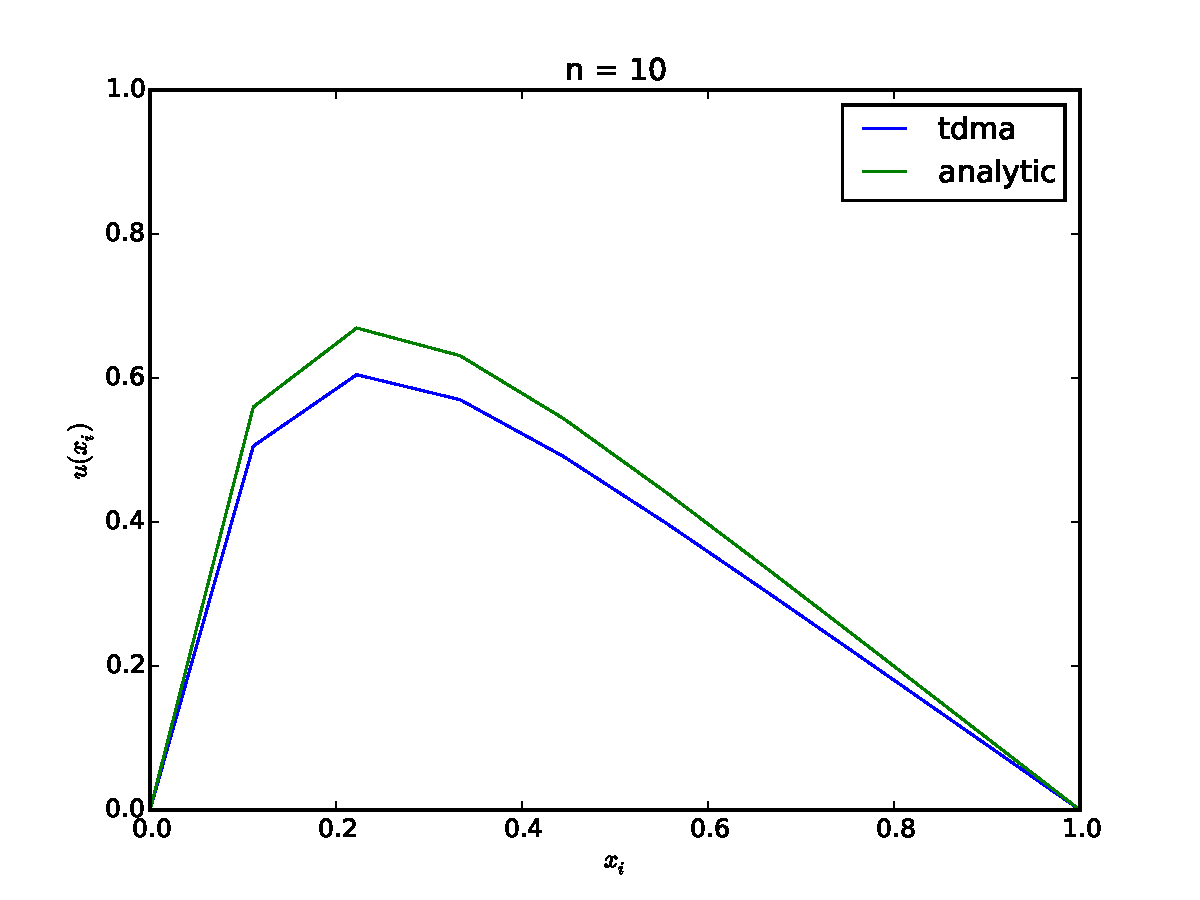
\includegraphics[width=\textwidth]{../plots/tdma_10} 
  \end{subfigure}
  \begin{subfigure}{0.3\textwidth}
    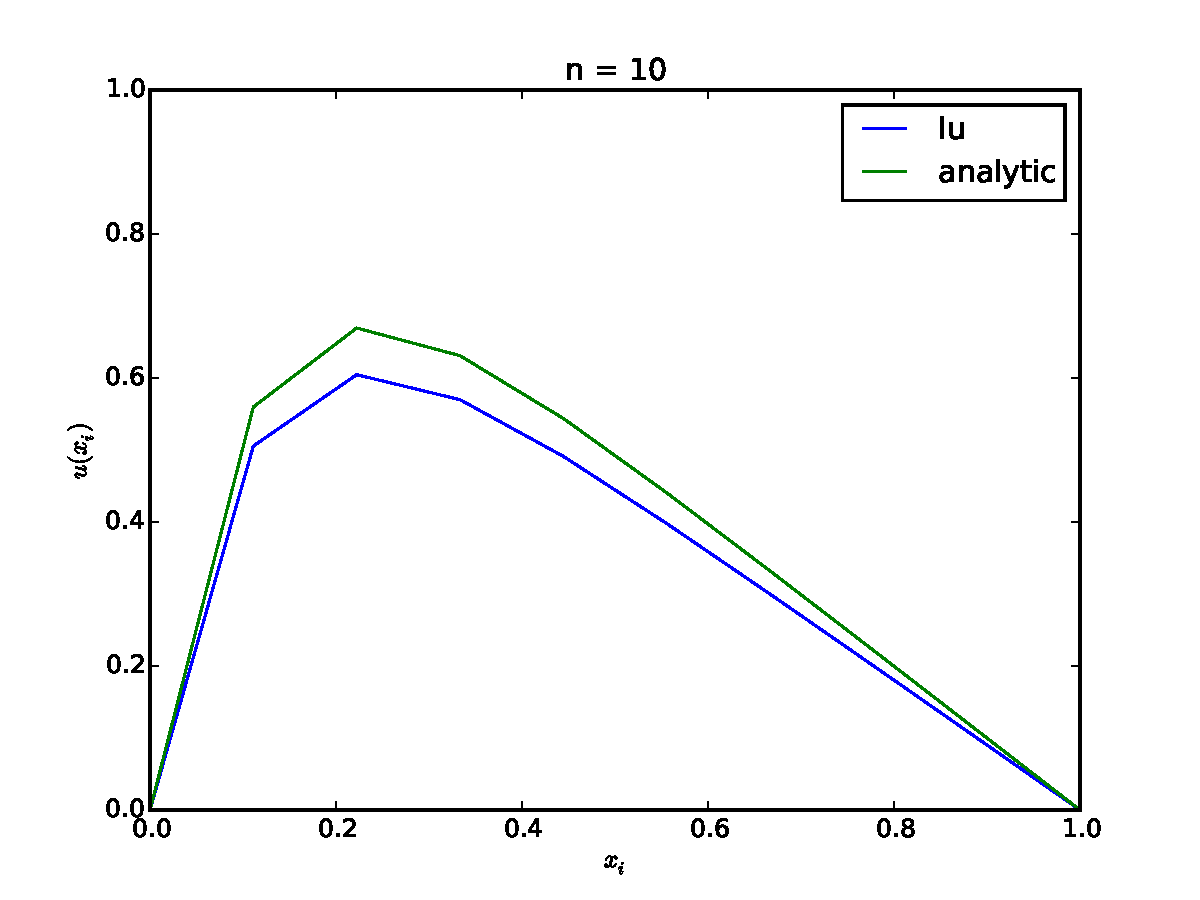
\includegraphics[width=\textwidth]{../plots/lu_10} 
  \end{subfigure}
  \\
  \begin{subfigure}{0.3\textwidth}
    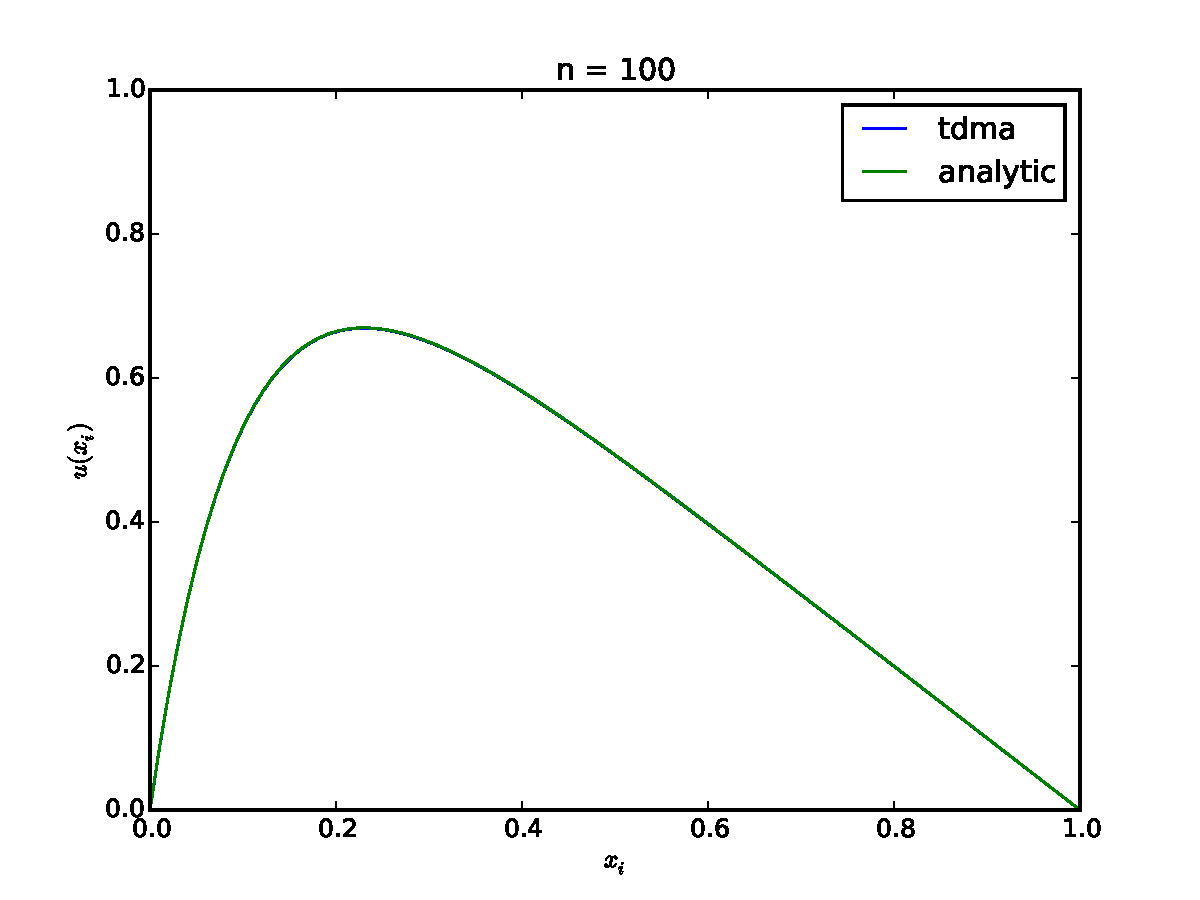
\includegraphics[width=\textwidth]{../plots/tdma_100} 
  \end{subfigure}
  \begin{subfigure}{0.3\textwidth}
    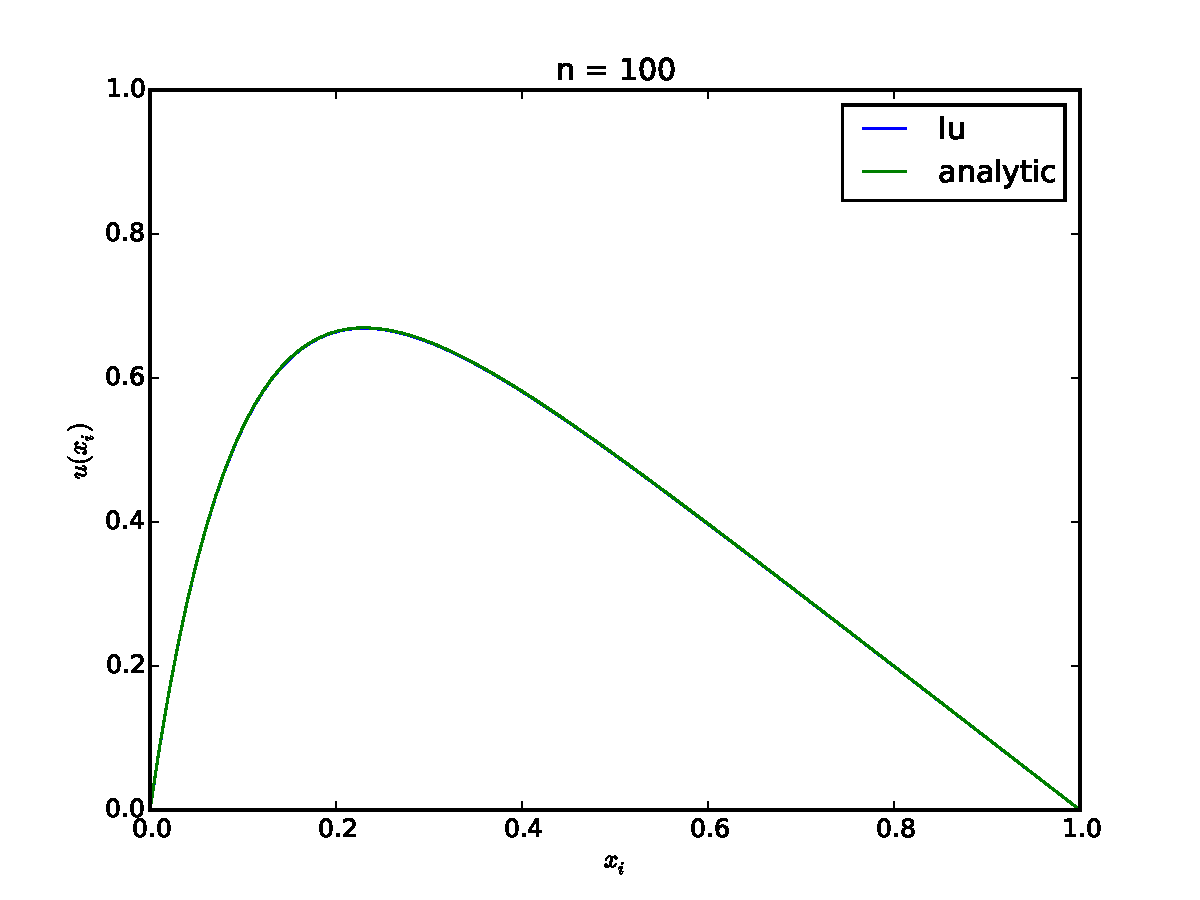
\includegraphics[width=\textwidth]{../plots/lu_100} 
  \end{subfigure}
  \\
  \begin{subfigure}{0.3\textwidth}
    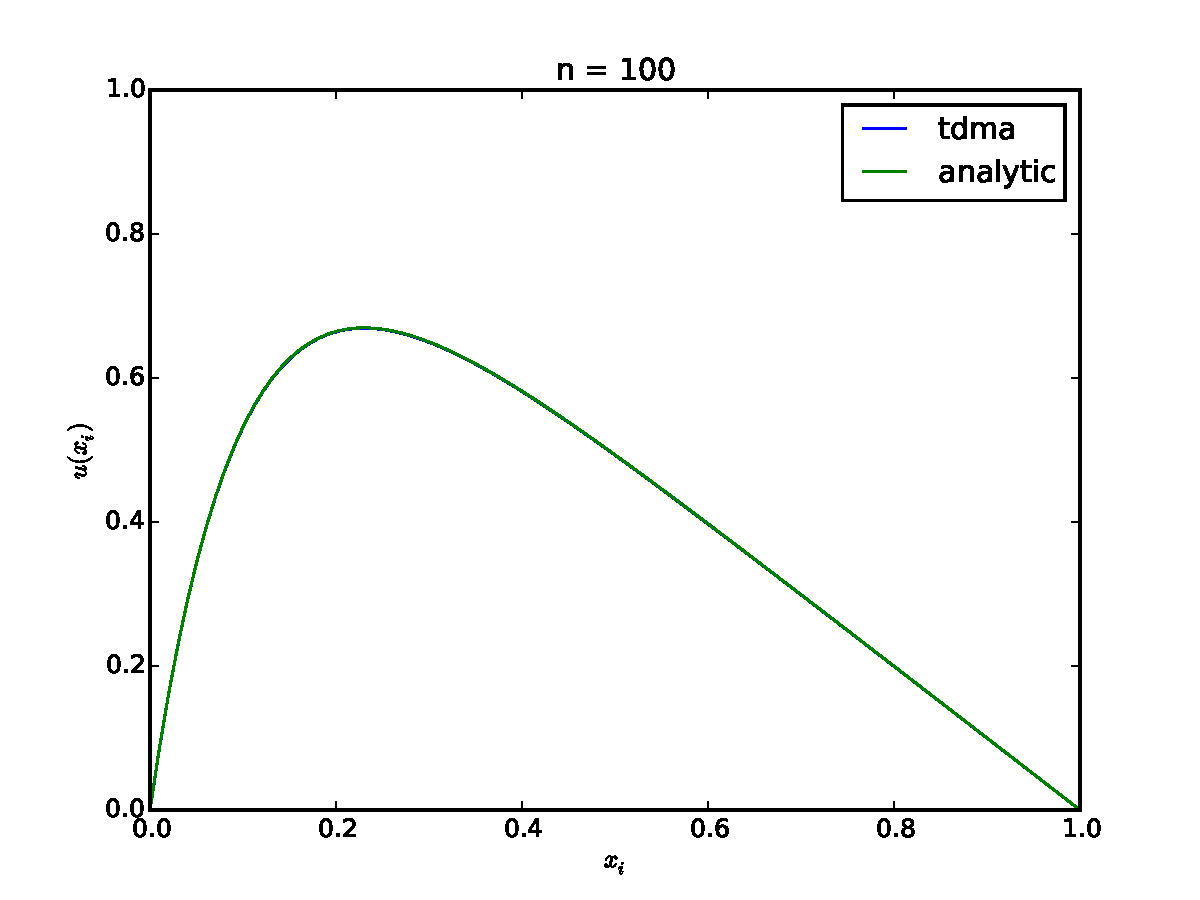
\includegraphics[width=\textwidth]{../plots/tdma_100} 
  \end{subfigure}
  \begin{subfigure}{0.3\textwidth}
    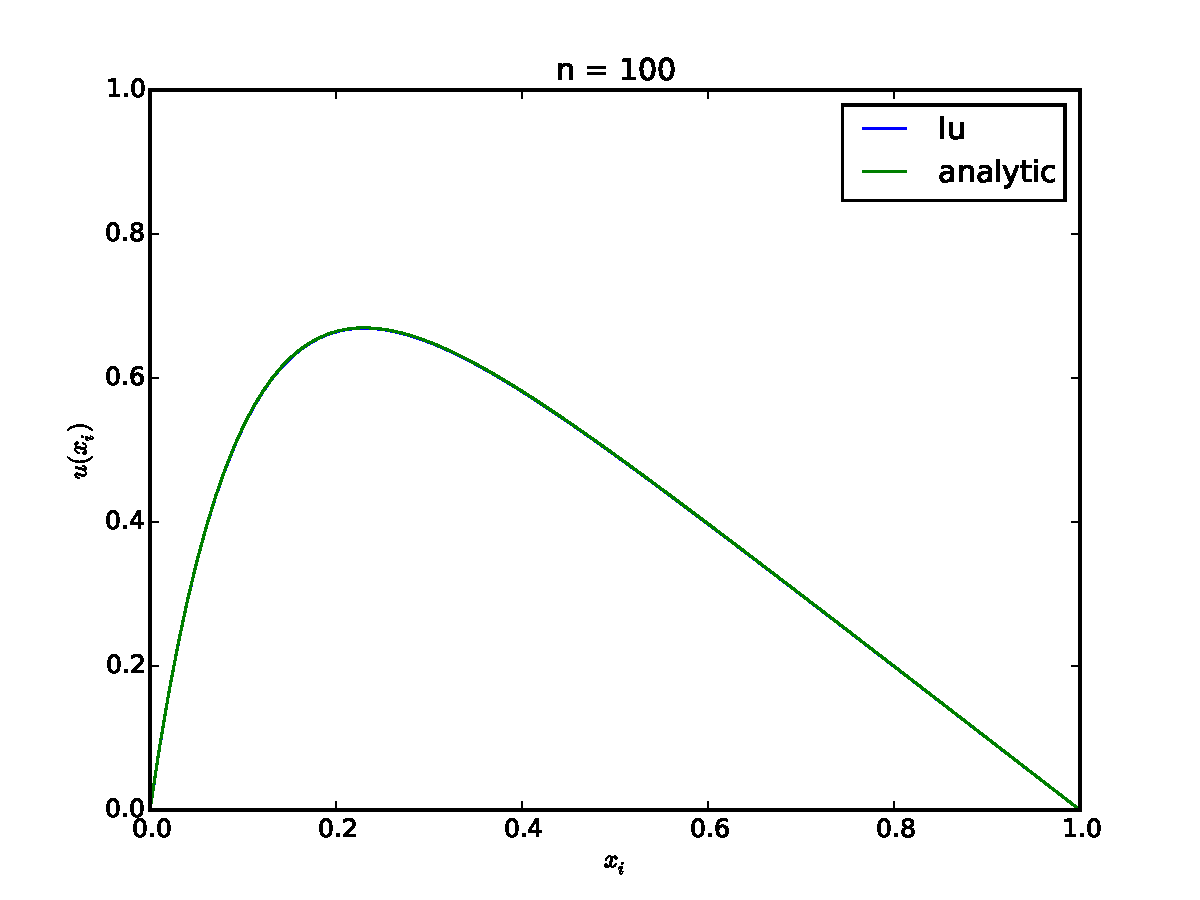
\includegraphics[width=\textwidth]{../plots/lu_100} 
  \end{subfigure}
\end{figure}

Of interest is also the relative error in our data set using the TDMA for various $n$. This has been computed and is presented in \cref{f:relerr}.

\begin{figure}[htb]
  \centering
  \caption{Relative error in dataset}
  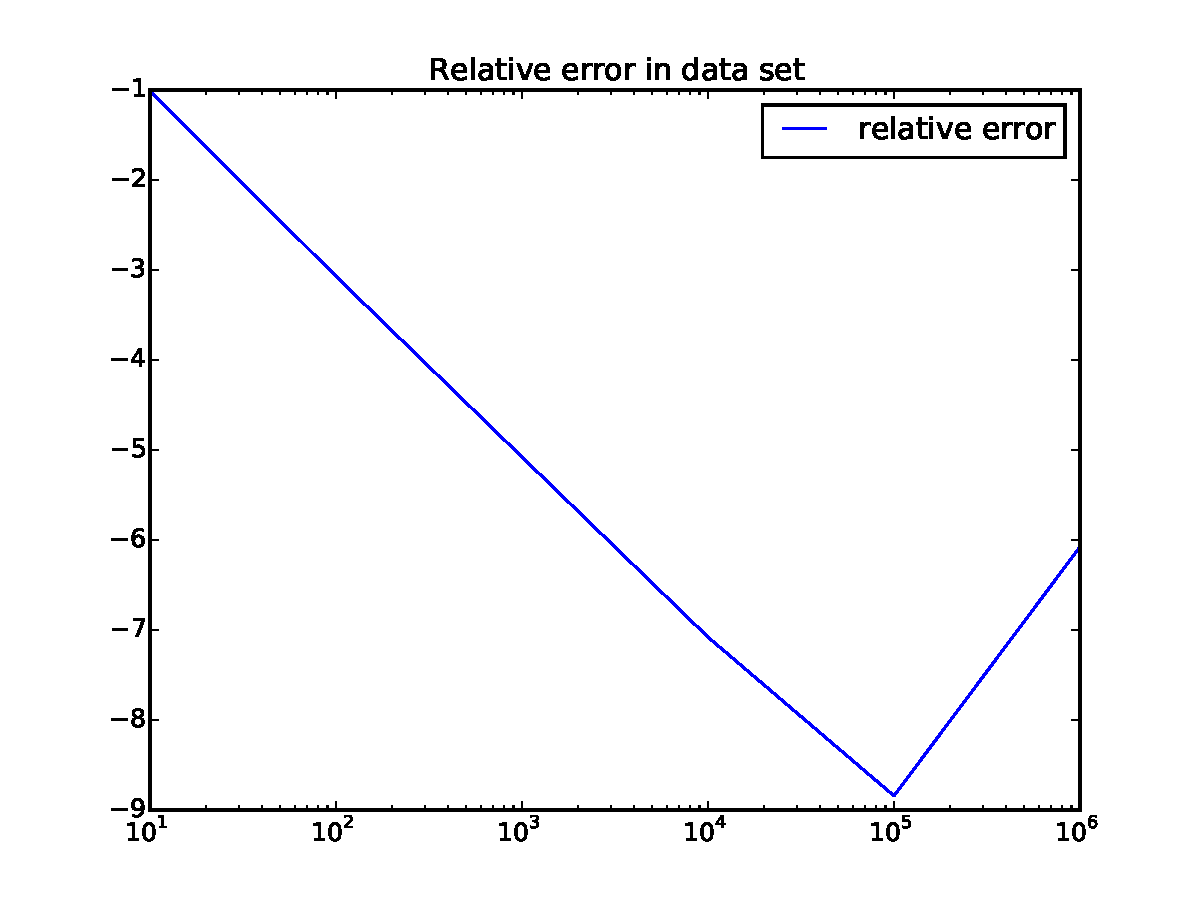
\includegraphics[width=0.8\linewidth]{../plots/relative_error}
  \label{f:relerr}
\end{figure}

The maximum relative error for each time-step is given in \cref{t:relerr_max}.
We see that at $n = 10^5$ the error start increasing again due to the error in
numerical precision becomes large as $h$ becomes small, as we can see in
\cref{eq:diff_app}.
\begin{table}[h]
\caption{Maximum relative error in data set for various $n$}
\begin{tabular}{lc} \\
\hline
$n$ & $\varepsilon_{\text{max}}$ \\
\hline
10 & -1.014000\\
100 & -3.070670\\
1000 & -5.078310\\
10000 & -7.079110\\
100000 & -8.842960\\
1000000 & -6.075510\\
\hline
\end{tabular}
\label{t:relerr_max}
\end{table}

\section{Conclusion}
\label{sec:conclusion}

Our implementation of the \emph{Tridiagonal Matrix Algorithm} improves vastly
on the standard \emph{Gaussian elimination method} and \emph{LU-decomposition}
if speed is to be considered.  However, our algorithm is just an optimization
of the latter methods for use with tridiagonal matrix problems. The main
difference between our TDMA and the LU-method we used for comparison is that
our TDMA is tailored to this specific problem, while the LU-decomposition
method in Armadillo is for a general case.  Hence the latter method is much
much slower. Other than that, the results are similar and no loss in numerical
precision occurs using the one over the other.

In addition, our TDMA is memorypreserving in the sense that it does not have to store each element of a sparse matrix, but just the diagonal vectors. We could even improve on this further, by observing that our diagonal vectors are constant. 

\subsection{Things to consider}
\label{sub:things_to_consider}

During this project I learned the importance of planning my implementation of a
numerical algorithm before starting to implement it. Knowing how to count, from
1 to $n$ is key. I struggled a bit with layout out the algorithm for the
boundary conditions as well as knowing what vector length to use. Having the algorithms
written down before starting to implement, as in Figure 1 and 2 helped a lot
and I`ll keep this in mind for the next projects. 

I also spent significant time debugging my \verb Python -implementation when the error was in the writing to file in my \verb C++ -program. 

\begin{thebibliography}{10}
  \bibitem{thomasalgo}{\textit{https://en.wikipedia.org/wiki/Tridiagonal\_matrix\_algorithm}}
  \bibitem{candh}{\textit{http://www.gocomics.com/calvinandhobbes/1986/11/26}}
  \bibitem{gauss}{\textit{https://en.wikipedia.org/wiki/Gaussian\_elimination\#Computational\_efficiency}}
  \bibitem{fys3150}{ \textit{Computational Physics - Lecture Notes Fall 2015 - Morten Hjorth-Jensen}}
\end{thebibliography}

\end{document}


